\chapter{Implementation}
-How implemented
\section{Approach}
\par The development approach focused on the business-logic, or back-end, of the system. From the two main development methodologies, Waterfall and Agile, the latter was used. In Waterfall, the development process is sequential. Development is a sequence of phases that are completed one after the other. When a stage is completed it is not returned to, as like with a Waterfall, it is not possible to go up to the previous stage (cite). Agile development focuses on adaptive planning, evolutionary development, and continuous improvement. The advantage of using an Agile approach over a Waterfall approach is that unpredicted features and issues are dealt with when they arise. This does make Agile difficult to manage, as there is no clear indication of when the project will be completed.
 
\par Scrum is an Agile approach that uses Sprint cycles, which are short development periods. In the development cycles, a set of features must be implemented and tested. Testing allows to ensure that when new features are developed, the older features continue to work as expected. At the end of each cycle, meetings are held discussing what are the next steps, and what issues arose during the previous cycle. For this project, the meetings were with the supervisor.
 
\par The Agile approach proved to be useful when a new timeline view had to be implemented. A clear example of the advantage of this system was when a new timeline view was suggested. In this new view, events are grouped by their start and end dates, such that events that occur within the period of other events are encapsulated by the longer event. This could be implemented in the system, due to the separation of the business logic and the view, and the development approach used. In a Waterfall model, the development is more structured, and thereby it is extremely useful for static requirements, i.e. requirements that will not change. However, in this case it would have caused issues in implementing the new view as it would require going up the Waterfall if the view of the system had already been implemented, or waiting until that step of the waterfall had been reached.

\par Note that the Agile methodology is used in software development teams. However,	 it can be applied to individual developments, since the structure of the project allows for sprint cycles and review meetings with the supervisor, as well the possibility of new requirements.

\section{Tools \& Software Libraries}
-development environment
-why used that environment
-software libraries (include an example use)
-why
\par The development environment of the project includes a 64-bit Windows 10 machine, with an Intel Core i7-6700HQ CPU at 2.60GHz and 16.0GB of Random Access Memory (RAM). It includes a Java Intelligent Development Environment (IDE), with Git for version-control, and Gradle for dependency management. 

\par The use of version-control allows development of features to be separated from the current working version of the code through the usage of branches. New features are added to the working version of the code, only if the required tests pass. Note this follows a Git flow development. In Git flow, a develop branch is made with the newest working features of the system, and new features are developed on separate branches. A master branch will only contain the latest fully implemented working version of the product. Using branches allows for bugs and development mistakes to be pin-pointed to the development of a specific feature, and allows the rollback to a previous, bug-free, state.

\par Gradle allows for libraries to be regarded as dependencies of the project. When the system is running on a separate machine, Gradle will retrieve the missing libraries used in the project before compiling and running the program. This allows for the system to be shared to other users, without having to include the libraries with the distribution of the code, as the required libraries and the version will be downloaded to the user's system when they run the command:
 \makebox[\textwidth]{ \textbf{gradlew run}.} 
Where gradlew is a wrapper for Gradle, such that the user does not even have to have Gradle installed in their system to run the application. Thereby, providing advantages in portability and general use.

\par As mentioned in the Background chapter, multiple libraries exist to aid the task of NLP. These are especially needed for the Named Entity Recognition(NER) and Text Summary tasks. An NER annotator will tag certain words, or collection of words into predefined categories such as People, Companies, Locations, and Money. These tools also aid in tagging words using the POS Treebank, which is a requirement to use the Hedge-Trimmer algorithm \cite{dorrzajicschwartz2003} to produce summaries. Using an NLP library speeds up the production of the system, as manually building an annotator requires multiple developers and years of work. As can be seen from the release history of the Stanford CoreNLP tool, development began in 2010 and the latest release was in 2016\footnote{\url{http://stanfordnlp.github.io/CoreNLP/history.html}}. The main two NLP tools available are Apache's OpenNLP\footnote{\url{https://opennlp.apache.org/}} and Stanford's CoreNLP\footnote{\url{http://stanfordnlp.github.io/CoreNLP/index.html}}. For this project, the Stanford's tool was used in the implementation, as it provides an extensive documentation and examples, along with specific sections describing their annotators in detail.

\par The Stanford tool is the main library used throughout the project, as the project is reliant on its NER and POS annotators (cite the stanford annotators). It comes with models, that are loaded during the initialisation of the system. These models are used in the statistical calculations in the annotators to determine whether certain words fall in predefined categories, or which POS tag should be given to them.

\par Due to the two main NLP libraries available being Java implementations, the decision was made to build the system in that language. It would be problematic to build the system in a different language to its libraries, as it would require making the two programming languages communicate with each other, which can cause unpredictable problems in the development and execution of the system.

\par Additional libraries in the development include JUnit for Unit testing. This allows for features to be tested. Testing is used in Git flow, to ensure that new features developed do not affect the correctness of older features, and are only merged together if the test succeed. Thereby, ensuring the system functions as expected.

\par Libraries for text extraction of .pdf and .docx file types are required, as the encoding of these files is not in plain text. The Apache POI\footnote{\url{https://poi.apache.org/}} and the Apache PDFBox\footnote{\url{https://pdfbox.apache.org/}} are used. In addition to text extraction, the PDFBox library along with the Apache Commons library allows the creation of PDFs (with text wrapping). This allows to save timelines as PDF documents. The Google GSON\footnote{\url{https://github.com/google/gson}} library is used for the creation of JSONs, to save the timeline in a JSON file. The RichTextFX\footnote{\url{https://github.com/TomasMikula/RichTextFX}} library along with JavaFX library are used to build the Graphical User Interface (GUI) of the system. It was ensured that the libraries used have licenses that allow their use in this project, and its later release to open-source.

\section{Issues}
\par Two main issues occurred during the implementation of the system: the creation of exact dates from named  entity dates, and the creation of an encapsulated timeline. A minor issue is also explained, which is based on the input documents being grammatically incorrect.

\subsection{Named Entity Recognition (NER) of Dates}
\par The Stanford CoreNLP tool, allows the resolution of temporal expressions. To explain this, an example is presented. The Stanford tool allows for reference dates to be used when a document is processed. When the tool tags a temporal expression as a DATE, it attempts to normalize it. Note the annotator treats each word in the sentence as a mention. To identify its named entity recognition tag, the following is done on the mention: \par
\makebox[\textwidth]{\textbf{mention.get(CoreAnnotations.NamedEntityTagAnnotation.class)}.}
If it is a temporal expression that was tagged, the result of the operation is a String DATE (to identify it as a date). Thus, from the mention, it can be normalized using: \par
\makebox[\textwidth]{\textbf{mention.get(CoreAnnotations.NormalizedNamedEntityTagAnnotation.class)}.}
The Stanford tool will attempt to produce a date in the ISO 8601\footnote{\url{https://www.cl.cam.ac.uk/~mgk25/iso-time.html}} format. As can be seen from the format, it can produce exact dates of the type dd-MM-yyyy, where dd is an integer value from 1 to 31, MM is the month as an integer value from 1 to 12, and yyyy the year. If BC dates are used, at the start of the normalized result a '-' is added (indicating a minus date). Using the ISO standard, an algorithm was written to process these dates. Note that, in addition to the possible dates given by the ISO standard, the Stanford tool produces 3 additional possible normalization outputs.

\par Normalizations refer to the attempt to produce a date from a temporal expression. It may be that, even with a reference point, the tool does not produce an exact date. For example, the temporal expression "now" would produce a normalized NER: "PRESENT\textunderscore REF", i.e. a reference to the present moment. For a temporal expression that refers to the past, e.g. "...they once used to...", "once" would be normalized to "PAST\textunderscore REF", i.e. a reference to the past of this moment. For a temporal expression that refers to the future, e.g. "In the future..., "future" would be normalized to "FUTURE\textunderscore REF", i.e. a reference to the future after this moment. 

\par The issue is that these normalizations do not allow for the comparison of events, which is required to sort them (as the start and end dates are not comparable). To allow for comparison, the most possible general dates for these references are derived. Since a "PRESENT\textunderscore REF" refers to the present moment, it can be deducted that it represents the moment in which the text was written in, as that is the time context in which the author wrote it. Thereby, the decision was made to produce as a general date for "PRESENT\textunderscore REF" a date that is the reference point provided by the user. As the reference point is supposed to be the date in which the text was written in. Note that the user can change the reference point to when-ever they would like, not just the assumed written date of the document. 

\par For "PAST\textunderscore REF" and "FUTURE\textunderscore REF" a range of dates is used, i.e. a start and end date. For the former, the start date of the era is used, i.e. 01-01-0001, and an end date to the reference point is used. This is because it can be determined that an ambiguous mention of the past would fall anywhere within that period, however an exact determination cannot be made due to the temporal expression not being precise enough. For the latter, the start date is the present moment, i.e. the base date, and the end date is the last possible allowable date in the system, i.e. 31-12-9999. This is because it would be appropriate for a mention of the future to refer to a moment between now (i.e. the present moment in which the text is presumed to be written in), and until the end of times. However, as a limitation to the system, the end of times is considered the date 31-12-9999. A snippet of the implementation of the algorithm is presented in Figure \ref{fig:refCode}.

\par Note that even though the Stanford CoreNLP library is well documented, it was difficult to find all the different outputs for the normalization of NER dates. It was after the discovery of Stanford's TimeML usage that a document describing the possible outputs of normalized NER dates was found\footnote{\url{http://www.timeml.org/timeMLdocs/TimeML.xsd}}. 

\begin{figure}[H]
\begin{lstlisting}
private ArrayList<Date> getDate(String date) {
	...
	/* Set up variables for processing */
	if (onlyPastRefPattern.matcher(date).matches()) {
            //past so make range from 0001-01-01 -> base date (range)
            if (yearMonthDayPattern.matcher(baseDate).matches()) {
                //base date has the format yyyy-MM-dd
               /*split it and set the values in date1, month1, year1 of 
		the start year 01-01-0001*/
		/*and the end date values of date2, month2, year2 
		to the base date data*/
		...
            }
        } else if (onlyPresentRefPattern.matcher(date).matches()) {
            if (yearMonthDayPattern.matcher(baseDate).matches()) {
                //base date has the format yyyy-MM-dd
		/*set day1, month1, year1 to the data in the base
		 date data*/
		...
            }
        } else if (onlyFutureRefPattern.matcher(date).matches()) {
            if (yearMonthDayPattern.matcher(baseDate).matches()) {
		//set the day1, month1, year1 to the base date data
            }
           //set year2, month2, day2 to the end year 31-12-9999
        }
	...
	/* date1, date2, month1 ,month2, year1, year2 are 
	then used appropriately to generate dates used 
	for the event that holds this Timeline Date */
}
\end{lstlisting}
\caption{Part of the Implementation of Resolution of Normalized NER Dates}
\label{fig:refCode}
\end{figure}

\subsection{Encapsulated Timeline View}
\par The initial representation of the events was a traditional timeline (see Figure \ref{fig:traditionalView}). This view is effective when the events are on separate time periods, as it presents them one after the other in a sequence. However, when there are multiple events that occur during the same period, they still appear one after the other. The issue is that unless the user specifically looks at the dates associated to the event, it is not possible for them to determine that the events occurred in the same period, but instead that one occurred after the other. This clearly violates the visibility objective of the system. A solution to this issue is to provide two views: the traditional timeline view which is effective at displaying events that have disjoint dates, and another view where the dates encapsulate the events. For example, if there is more than one event that occurs on the "25-01-2017", then instead of listing them both, one after the other, they are grouped visually by their date. However, visually grouping the events may lead to a "bin-packing" problem. The "bin-packing" problem consists of a set of bins, in this case a set of graphical views, which need to be fit in a finite space, in this case a box of fixed width and height. To deal with this issue, scrollbars can be used in the containers that hold the event layouts. Scrollbars allow for a container to be of infinite height (and/or width). Thus, being able to place the bins (graphical representations of events) in the container without considering the space limit. This view has been given the name "Range View". It requires placing the Results (the events of a set of documents) in Ranges (a data structure that can have one date, or a start and end date). The algorithm was discussed in the Design Chapter.

\begin{figure}[H]
\caption{Screenshot of the Traditional View of the Timeline of Events}
\label{fig:traditionalView}
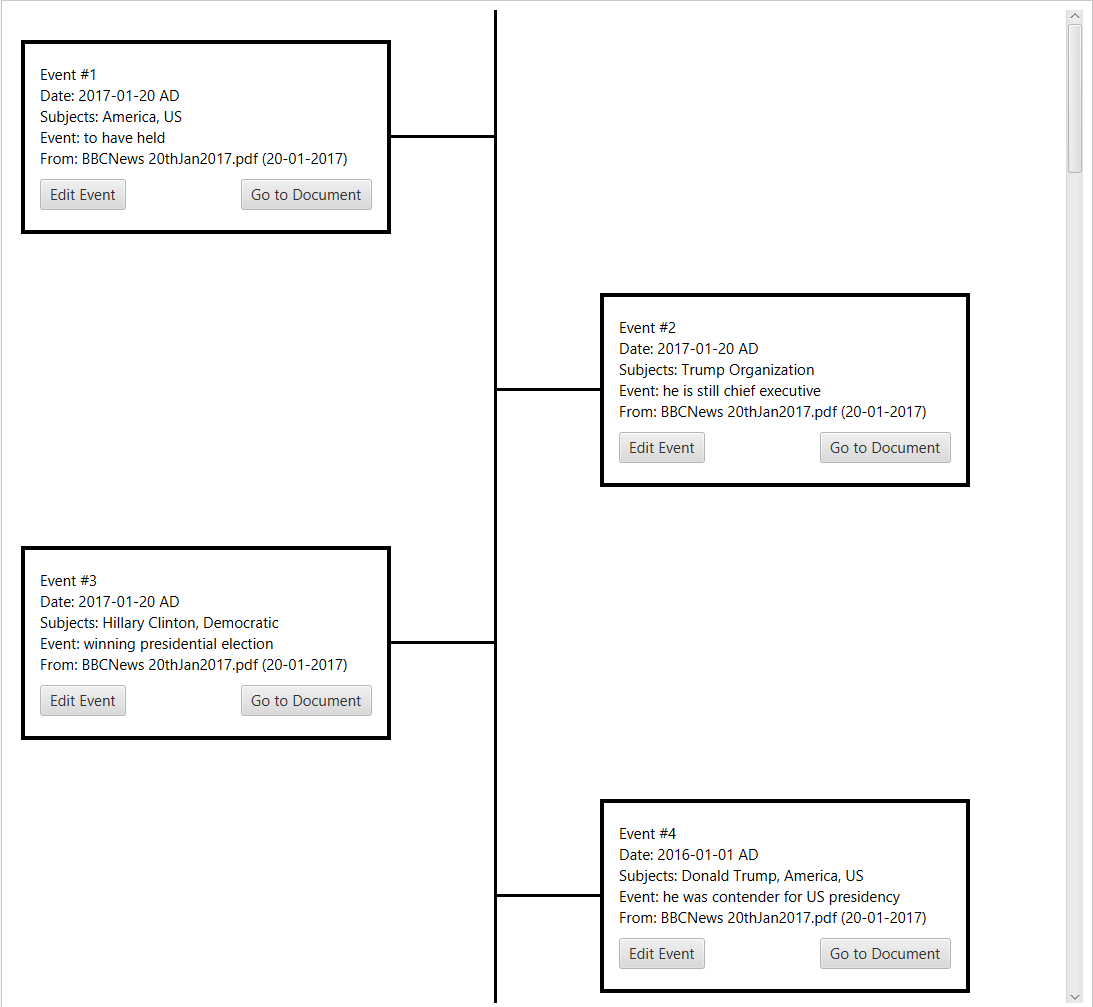
\includegraphics[width=\linewidth]{traditionalView.png}
\centering
\end{figure}

\par The algorithm behind the Range View, is having a list of Ranges, where each Range is a root node of a Tree of Ranges. Each Range may hold zero or more Results (i.e. events), and a set of children Ranges (zero or more). When the timeline needs to be produced, the list of Range roots is iterated over. The list of Ranges must have been sorted by their start date first. For each a GridPane is made. A GridPane is a layout which consists of rows and columns that can contain sub-views (where a sub-view is a view, i.e. a graphical component). In the first column, the current Range's data is placed (i.e. the date(s) and the Results held), and in the second column the layouts of the child Ranges are recursively set. The algorithm is presented in Figure \ref{alg:rangeLayout}. It is carried out for each Range root in the forest of Ranges.

\begin{algorithm}[H]
\underline{function getRangeLayout(list l)}\;
\SetKwInOut{Input}{Input}
\SetKwInOut{Output}{Output}
\Input{A list of Ranges, of size $n$, to add in the first column}
\Output{a layout that encapsulates the Ranges passed in the input, and their child Ranges}
GridPane toReturn\;
toReturn set the number of rows to the size of the input\;
toReturn set the number of columns $:= 2$\;
\For{i $:=$ 0 $\shortrightarrow$ n}{
	Range $:=$ input list at $i$\;
	set up layout for this Range, and set it in toReturn at position $(i,0)$\;
	set its column span at $(i,0)$ to remaining\;
	get layout for the children of this Range $:=$ getRangeLayout(range.children)\;
	set this layout in toReturn at position $(i,1)$\;
}
return toReturn\;
\caption{Pseudo-Code of the Recursive Production of the Range Layout}
\label{alg:rangeLayout}
\end{algorithm}

\par  In the implementation, it was decided to include 3 columns, to have a separator between a Range and its children. Thereby, improving the visibility of the timeline, as the user can differentiate between the Results of a range of dates, and the Results of a sub-range. The individual layout of a Range is listing the Results it holds, and the start and end date for this Range. An example look of the Range View can be found in Figure \ref{fig:rangeView}.

\begin{figure}[H]
\caption{Screenshot of the Range View of the Timeline of Events}
\label{fig:rangeView}
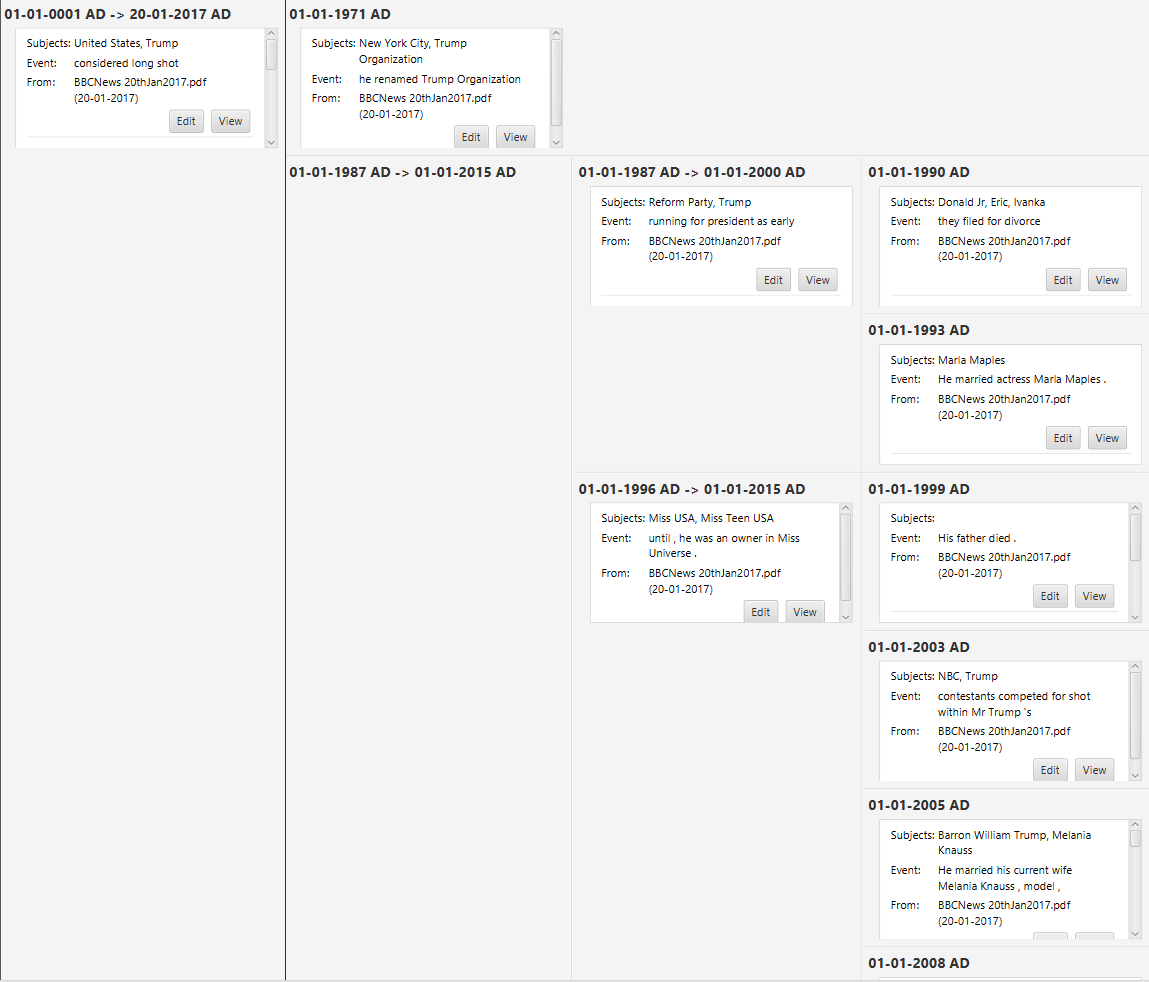
\includegraphics[width=\linewidth]{rangeView.png}
\centering
\end{figure}
\subsection{Incorrect Input Documents}

\par An important issue relating to the input documents is their format and grammar. NLP tools such as StanfordCoreNLP require certain constraints to be applied onto the input documents to be able to annotate them. These tools apply grammatical rules, thereby it is important that documents are grammatically correct to be able to correctly annotate them. This was discussed in the Background Chapter with a discussion on NLP tools being applied to Tweets. For this implementation, the documents are required to be in English as only the English models are loaded for the Stanford tool. The tool supports other languages\footnote{\url{http://stanfordnlp.github.io/CoreNLP/human-languages.html}} (such as German, and Spanish), however these require their own models. In addition, the algorithm applied to produce the summaries only works on English written text, as it uses the English grammar. In the future, the system can be extended to other languages.

\par An issue discovered, was that sentences that are separated by a period, but are not followed by a space, are treated as a single sentence. Thereby, it may be possible that only half the events are detected, if every two sentences are only separated by a period (and not a space). In addition, the summary would be applied to second sentence, as the rule of the algorithm details that the lowest-leftmost "S" subtree (i.e. sub-sentence) is picked. The start and end date, would therefore be the lowest date of the two events, and the highest date of the two events, due to how the dates of events are encapsulated in a TimelineDate object (that parses Normalized NER Dates, and updates the start and end dates it holds if a new minimum or maximum is found).

\par This issue cannot be prevented, as it would require manipulation of the input documents, and it can be the case that the user does not want the system to manipulate the input, but rather process it. Hence, it is advised to users to ensure the documents are in grammatically correct English, for the best results possible. Since the system will be used by law professionals, that are handling formal documents, it can be assumed that these documents would follow this format.
-ner dates (explain, then present how to solve it through examples of code)
-new timeline view (present how to solve it through examples of code)
-minor issue of incorrect text

\section{Testing}
\par Unit Tests were the testing focus in this project. A Unit Test is when individual units (or pairs) of source code of a system are tested to determine whether they are working correctly (cite). As the system was implemented in Java, the library used to aid this is JUnit\footnote{\url{http://junit.org/junit4/}}. Unit tests are primarily done on the back-end of a system, as the focus is on correctness in the logic, not in the UI. Automated tests carried out on the UI are called Instrumentation Tests. They involve emulating users' interaction with the system, i.e. pressing a button or filling in a text field. Both Unit and Instrumentation tests are automated, such that they are carried out one after the other without the involvement of the developer.

\par The reason as to why only Unit Tests were used, is that the systems primary focus is its processing of documents, and not its graphical representation. The representation is used to display the results; however, the system could also be used to process texts. Thus, the resulting intermediate JSON would be used in a third-party visual representation. Therefore, Instrumentation tests were not carried out.

\par A total of 35 tests were developed. The main advantage of these, is that when new features are developed, tests can be ran to ensure the rest of the system functions as expected. If the test cases are extensive and appropriate, then it can be assumed that the system will work correctly with the new features. In addition, this is aided using Git (in Git flow), where the features are developed on separate branches, and are only merged to the current working version of code if all the tests pass.

\par The focus was on the Engine (the component that takes as input text, and produces lists of Results), the processing of Files (test files were used in this case), the production of Ranges, the changing of the systems states throughout the processing task, the parsing of Normalized NER dates, and the production of JSON's from a list of Results (a timeline). Tests perform assertions. Assertions are when an actual output of code is checked with an expected output.

\par Tests were divided into three categories: a simple test, an intermediate test, and a complex test (where all possibilities of input are tested). For example, to produce Ranges, the complex test case expects multiple Range trees of different heights to be produced. Due to the benefit of Gradle, the tests can be ran using the command:\par
\makebox[\textwidth]{\textbf{gradlew test\footnote{after running gradlew build}}.}
In the build command, Gradle will not only run the test cases, but also produce the executable JAR which can be used to distribute the system as an executable to its non-developer users.

\section{UI}
//implementation ofthe UI.
\par From the wireframes presented in the Design Chapter, the actual User Interfaces(UI) was developed. The screenshots of the different windows are presented in the Figures below (see Figures \ref{fig:startUpImplemented}, \ref{fig:traditionalView}, \ref{fig:rangeView}, \ref{fig:editDialogImplemented}, and \ref{fig:viewDocImplemented}). Note that the interfaces provide the requested functionality through buttons and menus. Colour is missing as the focus was on functionality, visibility, and simplicity, instead of the UI being aesthetically pleasing. The system is aimed to be used for task completion, not enjoyment. The UI was, thus, developed to accomplish these tasks.

\begin{figure}[h]
\caption{Screenshot of the Start Up View}
\label{fig:startUpImplemented}
\includegraphics[width=\linewidth]{startUpImplemented.png}
\centering
\end{figure}
\begin{figure}[h]
\caption{Screenshot of the Edit Dialog View}
\label{fig:editDialogImplemented}
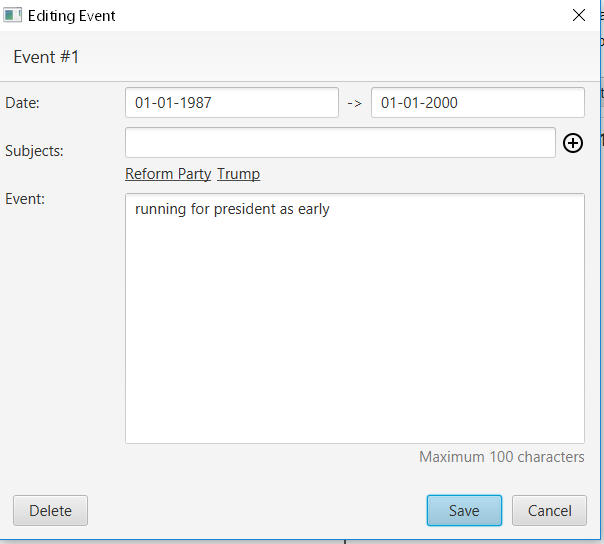
\includegraphics[width=\linewidth]{editDialogImplemented.png}
\centering
\end{figure}
\begin{figure}[h]
\caption{Screenshot of the Document Viewer}
\label{fig:viewDocImplemented}
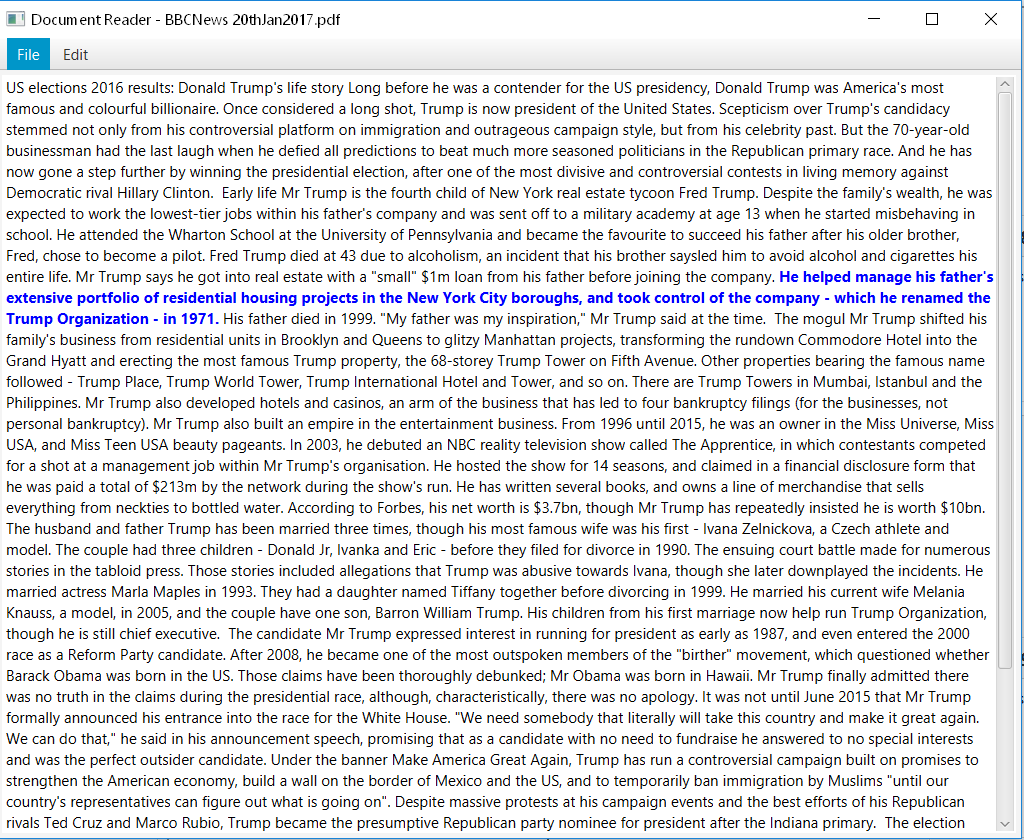
\includegraphics[width=\linewidth]{viewDocImplemented.png}
\centering
\end{figure}

\par Note that the Range view (see Figure \ref{fig:rangeView}) is zoomable (i.e. can zoom in/out). This allows the user to have a broader image of the Range View, if it is required. Therefore, allowing the user to obtain a general picture of what occurred.

\par The data presented of an event includes its subjects (key words) and summary. As the events are encapsulated in Ranges, it is sufficient to show the date(s) for the Range at the top. This demonstrates to the user that the following events occurred during that period.  This separates meta data (e.g. when an event occurred), from the actual event, which is what occurred in the event. Each event is accompanied by two buttons, the operations are: to edit the event (which includes deleting it, as can be seen from Figure \ref{fig:editDialogImplemented}), and viewing its document.

\par An advantage of the Traditional View over the Range view, is memory efficiency. Since the Range view has the function of being zoomable, due to programming language constraints, it cannot be implemented through a ListView. A ListView is a layout data structure where objects of a list are placed row by row. The ListView is memory efficient. It only produces the layout for a row when it needs to be shown. For example, for a list of 10000 items, it is very expensive to hold in memory the individual layouts of 10000 rows, especially if only 5 are being shown. Instead, only the 5 that are being shown are held in memory, and the rest are generated when needed. This is not the case with the Range View, due to it having the zoom function, and thus not being a ListView. As the memory capacity of personal computing systems (where the tool is intended to be used, but is not limited to) is large, this would not be an issue for the processing of tens or hundreds of events, however for larger sets this would cause memory issues. For large sets of events, the traditional view is recommended.

\section{Important Algorithms}
//highlight algorithm implementation: processing of files through semaphores, adding to ranges, pdf save and json save
\par This section presents note-worthy algorithms, in specific their implementation.
\subsection{Processing Files}
\par The pseudo-code of processing files was presented in the Design Chapter. The use of semaphores was also mentioned. Semaphores enforce that only $n$ processes can acquire their lock, with the $n+1$ process having to wait until another process releases its lock. However, the implementation is not trivial.

\par The system must allow a certain maximum number of threads to be ran in parallel to process documents. Processes must not fall in deadlock, which is when the processes are indefinitely allowing other processes to run, such that no run, or starve, which is when a process waits indefinitely to run. This can occur when semaphores are used, and they are not released when a process finishes its task. To ensure the semaphores are released, a call-back is given to the threads, which is to be used at the end of the threads parallel processing. If an error occurs, the semaphore is still released, allowing the next thread to run. Multi-threading precautions must be considered. When the call-back is used, data is also transferred (specifically the Results of processing the document) which can cause concurrency issues when two threads attempt to add a result list at the same time. Fortunately, Java provides the \textbf{synchronized} keyword for methods (see Figure \ref{fig:callbackFilesImplemented}). This ensures that no two threads may run the method at the same time. One thread must finish its execution of the method before another one can begin its execution.

%%Processing File was here
\begin{figure}[H]
\begin{lstlisting}
public synchronized void callBack(ArrayList<Result> results, FileData fileData) {
    //we finished processing a file
    filesToGo--;//one less to look at
    //add the results to the list held
    this.results.addAll(results);
    //release semaphore
    semaphore.release();
    //check if we have processed everything, 
    //if so release the finished semaphore
    if (filesToGo == 0) {
        //has processed
        BackEndSystem.getInstance().setSystemState(SystemState.PROCESSED);
        //has returned the results so we finished
        BackEndSystem.getInstance().setSystemState(SystemState.FINISHED);
        semaphoreFinished.release();
	    //value is now 1, so the thread that was acquiring can continue
    }
}
\end{lstlisting}
\caption{Implementation of call-back after Files have been processed}
\label{fig:callbackFilesImplemented}
\end{figure}

\par Threading precautions have been taken throughout the project. Where threads process sets of data, it was ensured that the data items in the set can be processed independently of each other. This cannot be possible in all situations, in such cases synchronization and semaphores are used to ensure concurrency.

\subsection{Building Ranges}
\par The algorithm for building Ranges out of Results was presented in the Design Chapter. However, it was not described how it can is checked if a Result can be added to an existing Range. When a Result is attempted to be added to a pre-existing Range, an \textbf{add()} (see Figure \ref{fig:addRangeImplementation}) method is called. In this method, it is initially checked whether the Result should be added to this Range. This check involves looking at the dates of the Result and checking whether the Range's dates fully or partially encapsulate them. If this is not the case, then the attempt of adding the Result fails. If the Range encapsulates the Result's dates then it will be checked whether the Result can be added to any of the nodes of the Range tree. This would occur if there is any node in the tree that holds the same exact dates as the Result. If this is the case then the Result will be added to that node. If this is not the case, then it can be determined that the Result belongs to this Range, however its position in the tree needs to be created. It can be the case that there is a Range that partially encapsulates the Result, if so the Range would need to be expanded. In both cases, the tree needs to be traversed to find the optimal position for the Result.

\begin{figure}[H]
\begin{lstlisting}
public boolean add(Result result) {
    TimelineDate timelineDate = result.getTimelineDate();
    //check constraints
    if (!shouldAdd(timelineDate)) {
	//check constraints if we can even add to this range
        return false;
    }
    //attempt to add through an existing range
    Range toAdd = checkCanAdd(result);
    if (toAdd != null) {
	//add to the results of the given range
        toAdd.results.add(result);
        return true;
    }
    //now we try to extend the range
    return createRangeAndAdd(result);
}
\end{lstlisting}
\caption{Implementation of Adding Results to a Range}
\label{fig:addRangeImplementation}
\end{figure}

\subsection{Saving Results}
\par Saving the results of the processed documents, is divided into two parts: saving them as a PDF, or as a JSON. 

\par In the PDF, the file that is saved, is a graphical representation of the events, using the traditional timeline view. It is aided by the Apache PDFBox and Commons library. The libraries work like a painting tool. The pages are canvases, where lines and text can be drawn on at specific positions. These positions are given by coordinates $(x,y)$, where the top left of the page is the origin, i.e. $(0,0)$, and the $x$ values increment towards the right of the page, and the $y$ values towards the bottom of the page. To build a dynamic system, that can create a pdf for any number of Results, certain constraints are required. For example, the maximum number of events to be displayed on each page, and the size of the text of the summaries and subjects (i.e. how many characters). Due to tool limits, it is not possible to continue drawing on the next page of the PDF document, hence events cannot overflow onto the next page. However, since the text that is used in the summary should be short, assumptions can be made. For example, the maximum size of a container that holds an event. Knowing this, it allows the drawing of containers of maximum size on the document. Thus, ensuring that all the data for each event will fit in a container. Therefore, the system can be considered as drawing containers on the page and filling them with their event data. This is repeated for all the events, and where necessary creating a new PDF page to fill more events. Hence the task, has been broken down to moving the $x$ and $y$ positions, writing text (the event data), and drawing the rectangle (container). Since in the traditional view, the layout of the events is one on the left of the page and the other on the right of the page, the tasks must be changed minimally to allow for this. In Figure \ref{fig:drawRecImplemented}, the implementation, to draw an event on the right of the page, is provided.

\begin{figure}[H]
\begin{lstlisting}
private void drawOddEvent(Result result, PDPageContentStream contentStream, int position) throws IOException {
	//initially y is the top right where this needs to 
	//be shown, x starts from the middle
	currentY -= padding; //add some padding to y
	currentX = (int) widthOfPage / 2;
	contentStream.moveTo(currentX, currentY);
	//write the text for the Event
	int lengthOfHorLine = (int) ((widthOfPage / 2) - (padding + widthOfRectangle));
	currentX += lengthOfHorLine;
	writeText(result, contentStream, currentX, position);
	//draw the rectangle to surround the text
	drawRectangle(contentStream, currentX, currentY - heightOfRectangle);
	//draw the horizontal line connecting event timeline
	currentY -= heightOfRectangle / 2;
	contentStream.moveTo(currentX, currentY);
	contentStream.lineTo(widthOfPage / 2, currentY);
	contentStream.stroke();
	currentY -= (heightOfRectangle / 2) + padding;
}
\end{lstlisting}
\caption{Implementation of drawing for a Result in the PDF timeline}
\label{fig:drawRecImplemented}
\end{figure}

\par The JSON implementation, is aided using the Google GSON library. JSON provides a clearly defined key-value data format that can be interpreted by any system. The advantage of this library is that it allows for a flexible creation of JSONs. Specifically, it allows the developer to specify how an object of a given type should be serialized (see Figure \ref{fig:adapterGsonImplemented}), i.e. how its data should be extracted into JSON format. In this case, the objects to be serialized are Result objects. The data extracted from a Result includes its start and end date, its list of subjects, its summary, and its file data. This is done through an adapter. The adapter defines how the data of the Result object is extracted, and how a JSON Object is created. For a list of Results, this will be carried out for each Result, and thereby, a resulting list of JsonObjects will be produced, i.e. a JsonArray. This can then be saved by the user in a file, and can then be interpreted by any third-party system. The format of a JSON of a Result is given in Figure \ref{fig:jsonResult}. Where G, in the dates, is the ERA (i.e. BC or AD) of the date.

\begin{figure}[h]
\begin{lstlisting}
{
"date1":dd-MM-yyyy G,
"date2":dd-MM-yyyy G,
"subjects":[],
"event":String,
"from":{
	"filename":String,
	"baseDate":dd-MM-yyyy
	}
}
\end{lstlisting}
\caption{Structure of Result (event) JSON}
\label{fig:jsonResult}
\end{figure}
\begin{figure}[H]
\begin{lstlisting}
public JsonElement serialize(Result src, Type typeOfSrc, JsonSerializationContext context) {
	//json object for this result
    	JsonObject jsonObject = new JsonObject();
	//adding the range dates (which can be null)
	/* whenever a value is null, the key-pair will not be included in the final JSON */
	jsonObject.addProperty("date1", src.getTimelineDate().getDate1FormattedDayMonthYear());
	jsonObject.addProperty("date2", src.getTimelineDate().getDate2FormattedDayMonthYear());
	//adding the subjects
	JsonArray subjectJsonArray = new JsonArray();
	for (String subject : src.getSubjects()) {
		subjectJsonArray.add(subject);
	}
	jsonObject.add("subjects", subjectJsonArray);
	//adding the event
	jsonObject.addProperty("event", src.getEvent());
	/*adding the file data (excluding the path, since this can be used on other system where files are elsewhere)*/
	JsonObject fromJsonObject = new JsonObject();
	FileData fileData = src.getFileData();
	if (fileData != null) {
		fromJsonObject.addProperty("filename", fileData.getFileName());
		fromJsonObject.addProperty("baseDate", fileData.getCreationDateFormattedDayMonthYear());
	}
	jsonObject.add("from", fromJsonObject);
	return jsonObject;
}
\end{lstlisting}
\caption{Implementation of the Serializer used in the Adapter to generate JSON for a list of Results}
\label{fig:adapterGsonImplemented}
\end{figure}

-main algorithms: for building events, building ranges, pdf save, json save, processing files
